
\subsection{Model}

The Hubbard model\cite{Montorsi1992} describes spin-$\frac{1}{2}$ fermions with a local interaction:
\begin{equation}
 \mathcal{H} = \sum_{i,j,\sigma} t_{ij} c^{\dagger}_{i,\sigma} c_{j,\sigma}
 + U \sum_{i} n_{i,\uparrow} n_{i,\downarrow} ,
\end{equation}
where $c^{\dagger}_{i,\sigma}$ ($c_{i,\sigma}$)  creates (annihilates) a fermion on site $i$ with spin orientation $\sigma$ ($\uparrow$ or $\downarrow$). We consider the two-dimensional case on a square lattice and repulsive interaction $U>0$ at finite temperature $T$. The hopping amplitude is restricted to $t_{ij} = -t$ for nearest neighbors, $t_{ij}=-t'$ for next-to-nearest neighbors. Fourier transforming the hopping matrix yields the bare dispersion relation
\begin{equation}
 \varepsilon_{\mathbf{k}} =
 -2t \left( \cos{k_x} + \cos{k_y} \right) -4 t' \cos{k_x} \cos{k_y} .
\end{equation}


\subsection{Flow equations}

In the following paragraph we will provide some details about the functional renormalization group for interacting fermion systems,\cite{Metzner2012,Platt2013} defining in particular the notation used for the vertex. 

The fRG implements a scale-by-scale evaluation of the functional integral describing the many-body system. 
This is done by endowing the bare action with an additional dependence on a scale-parameter $\Lambda$,
\begin{equation}
 \mathcal{S}^\Lambda[\overline\psi,\psi] =
 -(\overline\psi,{G_0^\Lambda}^{-1}\psi)+\mathcal{S}_{\mathrm{int}},  
\end{equation} 
where $\mathcal{S}_{\mathrm{int}}$ is the interaction part, and $(\overline\psi,\psi)$ denotes the summation over all the quantum numbers of the fermionic fields  $\overline \psi$ and $\psi$. 
The scale dependence, acquired through the non-interacting propagator $G_0^\Lambda$, generates flow equations (with known initial conditions) for generating functionals. These are defined via functional integrals with the action $\mathcal{S}^\Lambda$. 
Examples are the generating functional for the connected Green's function and its Legendre transform, the so-called average effective action.\cite{Wetterich1993}
The final result is recovered for some final $\Lambda$-value restoring the original bare propagator, $G_0^{\Lambda_\mathrm{f}} = G_0$, so that the physical action of interest is recoved.  

We will apply this approach to the effective action, whose expansions in the fields generates the one-particle irreducible (1PI) vertex functions. By expanding the functional flow equation,\cite{Wetterich1993} one obtains a hierarchy of flow equations for the 1PI functions, involving vertices of arbitrarily  high orders. 
We will restrict ourselves to the two-particle level truncation by retaining only the two lowest nonvanishing orders in the expansion, that is, we consider the flow of the self-energy $\Sigma^\Lambda$ and of the two-particle vertex $V^\Lambda$, neglecting the effects of higher order vertices. 
This truncation restricts the applicability of the approach to the weak-to-moderate coupling regime.\cite{Salmhofer2001} 
It can be further shown that, at the two-particle level trunctaion, the fRG sums up efficiently, although approximately, the so-called parquet-diagrams.\cite{Kugler2017}
  
Due to SU(2) symmetry, the self-energy is diagonal in spin-space: 
\begin{equation}
\Sigma^\Lambda_{\sigma\sigma'}(k)=\Sigma(k)\delta_{\sigma,\sigma'}, 
\end{equation}
where $k=(\mathbf{k},\nu)$, $\nu$ is a fermionic Matsubara frequency and $\mathbf{k}$ a momentum in the first Brillouin zone. 
\begin{figure}[t!]
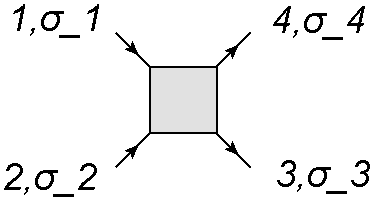
\includegraphics[width=0.2\textwidth]{images/VertexBox.png}
\caption{Notation of the two-particle vertex.} 
\label{fig:notvert} 
\end{figure}

For the notation of the two-particle vertex function $V_{\sigma_1\sigma_2\sigma_3\sigma_4}(k_1,k_2,k_3)$ we refer to Fig.~\ref{fig:notvert}, where $k_i=(\mathbf{k_i},\nu_i)$.
The momentum $k_4=k_1+k_2-k_3$ is fixed by momentum conservation.
The SU(2) spin-rotation symmetry guarantees that the vertex vanishes for all the six spin combinations apart from six:
$V^\Lambda_{\uparrow\uparrow\uparrow\uparrow} =
 V^\Lambda_{\downarrow\downarrow\downarrow\downarrow}$, 
$V^\Lambda_{\uparrow\downarrow\uparrow\downarrow} =
 V^\Lambda_{\downarrow\uparrow\downarrow\uparrow}$, and
$V^\Lambda_{\uparrow\downarrow\downarrow\uparrow } =
 V^\Lambda_{\downarrow\uparrow\uparrow\downarrow}$.   
Finally, due to SU(2) symmetry and crossing relation one has \cite{Rohringer2012} 
\begin{eqnarray}
\nonumber
V^\Lambda_{\uparrow\uparrow\uparrow\uparrow}(k_1,k_2,k_3) &=& V^\Lambda_{\uparrow\downarrow\uparrow\downarrow}(k_1,k_2,k_3)\\&-& V^\Lambda_{\uparrow\downarrow\uparrow\downarrow}(k_1,k_2,k_1+k_2-k_3),
\label{eq:spinsym1}
 \\ 
V^\Lambda_{\uparrow\downarrow\downarrow\uparrow}(k_1,k_2,k_3)& =& -V^\Lambda_{\uparrow\downarrow\uparrow\downarrow}(k_1,k_2,k_1+k_2-k_3).
\label{eq:spinsym2}
\end{eqnarray}
This allows us to express the vertex by only one function of three frequency-momentum arguments: $V^\Lambda(k_1,k_2,k_3)\equiv V^\Lambda_{\uparrow\downarrow\uparrow\downarrow}(k_1,k_2,k_3)$ where all the others spin components are obtained by Eqs.~(\ref{eq:spinsym1}-\ref{eq:spinsym2}).\cite{Husemann2009}

The flow equation for the self energy can then be written as \cite{Metzner2012} 
\begin{equation}
\frac{d}{d \Lambda} \Sigma^\Lambda(k)= -\int_p  S^\Lambda(p)\left[2V^\Lambda(k,p,p) -V^\Lambda(k,p,k)\right], 
\end{equation}
with $p=(\mathbf{p},\omega)$ and $k = (\mathbf{k},\nu)$.
We use the notation  $\int_{p} = T \sum_\omega \int_{\mathbf{p}}$, where $\sum_\omega$ is the Matsubara frequency sum, and $\int_{\mathbf{p}}=\int  \frac{d\mathbf{p}}{(2\pi)^2}$ is the normalized integration over the first Brillouin zone. 
\begin{equation}
 S^\Lambda = \left. \frac{dG^\Lambda}{d\Lambda}\right|_{\Sigma^{\Lambda}=\mathrm{const}} 
\end{equation}
is the socalled single-scale propagator, and ${G^\Lambda}$ is the full propagator, which is related to the bare propagator and the self-energy by the Dyson equation
$(G^\Lambda)^{-1} = (G_0^\Lambda)^{-1} - \Sigma^\Lambda$. 
  
\begin{widetext} 
The flow equation for the vertex can be written as \cite{Metzner2012, Husemann2009}
\begin{align}
\label{eq:vertflow}
 \frac{d}{d\Lambda}V^\Lambda(k_1,k_2,k_3) = \fl{\mathcal{T}}{pp}(k_1,k_2,k_3) +  
  \fl{\mathcal{T}}{ph}(k_1,k_2,k_3) + \fl{\mathcal{T}}{phc}(k_1,k_2,k_3),
\end{align} 
where \footnote{The equation for the particle-particle channel is slightly different from the one usually reported in fRG, see, e.g., Ref.~\onlinecite{Husemann2009}. This is because we took $\fl{V}{} = \fl{V}{\uparrow \downarrow \uparrow\downarrow}$ instead of $\fl{V}{} = \fl{V}{\uparrow\downarrow\downarrow\uparrow}$.}
\begin{eqnarray}
\label{eq:ppT} 
\fl{\mathcal{T}}{pp}(k_1,k_2,k_3) &=&-\frac{1}{2} \int_p \fl{\mathcal{P}}{\mathrm{pp}}(k_1+k_2,p) \Big\{  \fl{V}{}(k_1,k_2,k_1+k_2-p)\fl{V}{}(k_1+k_2-p,p,k_3) 
\label{eq:tpp} 
   \\ 
\nonumber
&&+  \fl{V}{}(k_1,k_2,p)\fl{V}{}(p,k_1+k_2-p,k_3) \Big\} , \\  
\label{eq:tph} 
\fl{\mathcal{T} } {ph}(k_1,k_2,k_3) & =& -\int_p \fl{\mathcal{P}}{\mathrm{ph}}(k_3-k_1,p)
\Big\{ 2 \fl{V}{}( k_1,k_3-k_1+p,k_3)  \fl{V}{}(p,k_2,k_3-k_1+p) \\
\nonumber
&&- \fl{V}{}( k_1,k_3-k_1+p,p)  \fl{V}{}(p,k_2,k_3-k_1+p) - \fl{V}{}( k_1,k_3-k_1+p,k_3)  \fl{V}{}(k_2,p,k_3-k_1+p) \Big\} , \\
\label{eq:tphc}
\fl{\mathcal{T}}{phc}(k_1,k_2,k_3) & =& \int_p \fl{\mathcal{P}}{\mathrm{ph}}(k_2-k_3,p) \fl{V}{}(k_1,k_2-k_3+p,p)
\fl{V}{}(p,k_2,k_3).
\end{eqnarray} 
\end{widetext}
Here $\mathcal{T}^\Lambda_{\mathrm{pp}}$, $\mathcal{T}^\Lambda_{\mathrm{ph}}$ and $\mathcal{T}^\Lambda_{\mathrm{phc}}$ stand respectively for \textit{particle-particle}, \textit{particle-hole} and \textit{particle-hole crossed} contributions.
We have defined the quantities
\begin{align}
 \mathcal{P}_{\mathrm{ph}}^\Lambda(Q,p) &= G^\Lambda(Q+p)S^\Lambda(p) + G^\Lambda(p) S^\Lambda(Q+p), \\ 
 \mathcal{P}_{\mathrm{pp}}^\Lambda(Q,p) &=G^\Lambda(Q-p)S^\Lambda(p) + G^\Lambda(p) S^\Lambda(Q-p) ,
\end{align} 
which are the scale derivatives, at fixed self-energy, of the product of two Green's functions.

\subsection{Interaction flow}
\label{sec:IntFlow}
To use the flow equations defined above we need to specify the $\Lambda$-dependence of the non-interacting propagator $G_0^\Lambda$.
We use the \textit{interaction cutoff}, introduced by Honerkamp {\em et al.}: \cite{Honerkamp2004}
 \begin{equation}
 G_0^\Lambda(k) = \Lambda G_0(k) =
 \frac{\Lambda}{i\nu + \mu^\Lambda - \varepsilon_{\mathbf{k}}} , 
 \end{equation}
where the scale-parameter $\Lambda$ flows from $0$ to $1$. 
We have introduced a $\Lambda$-dependent chemical potential to maintain the density fixed during the flow.
The Dyson equation yields the interacting Green's function in the form
\begin{equation}
 G^\Lambda (k) = \frac{\Lambda}{i\nu - \varepsilon_{\bs{k}}
 + \mu^{\Lambda} - \Lambda\Sigma^\Lambda(k)} . 
\end{equation}
The scale-dependent chemical potential $\mu^\Lambda$ is determined from the equation
\begin{equation}
n = n^{\Lambda}(\mu^\Lambda) \equiv 2 \int_k \frac{e^{i\nu 0^{+}}} {i\nu - \varepsilon_{\bs{k}} +\mu^{\Lambda}-\Lambda\Sigma^\Lambda(k)}. 
\end{equation} 
The factor 2 accounts for the spin degree of freedom.

The main advantage of the interaction cutoff is that  the $\Lambda$-dependent action can be interpreted \cite{Honerkamp2004} as the physical action of the system with a rescaled interaction $U^\Lambda = \Lambda^2 U$.
Since $T$ acts as an infrared cutoff, for our purposes we do not need to worry about the fact that this cutoff is not scale-selective, and hence does not regularize possible divergences in the bubbles. 

%As a benchmark for the robustness of our results on the cutoff-choice, we have used a soft version of the \textit{frequency selective cutoff} defined\cite{Eberlein2014} by:
%\begin{equation}
%G_0^\Lambda(k) = \frac{1}{i\mathrm{sign}\sqrt{\nu^2+\Lambda^2 }-\mu- \varepsilon_{\bs{k}}},  
%\end{equation}  
%with $\Lambda_0=\infty$ and $\Lambda_{\mathrm{f}}=0$. Also in this case we have performed our calculations at fixed occupation. 


%For both our cutoff choices at the beginning of the flow one has $G_0^{\Lambda_0}=0$, corresponding to a initial conditions for the self-energy and the vertex  defined by, $\Sigma^{\Lambda_0}=0$ and $V^{\Lambda_0 }= U$. 
 


